\subsection{arithmetic\_extension}

To understand the design principle of this Gate, we must first understand \href{https://en.wikipedia.org/wiki/Field_extension#Extension_field}{Field extension}. 


Taking Plonky2's GoldilocksField as an example, we give the extension field elements under quadratic, quadratic and quintuple expansions respectively:

\begin{figure}[!h]
    \centering
    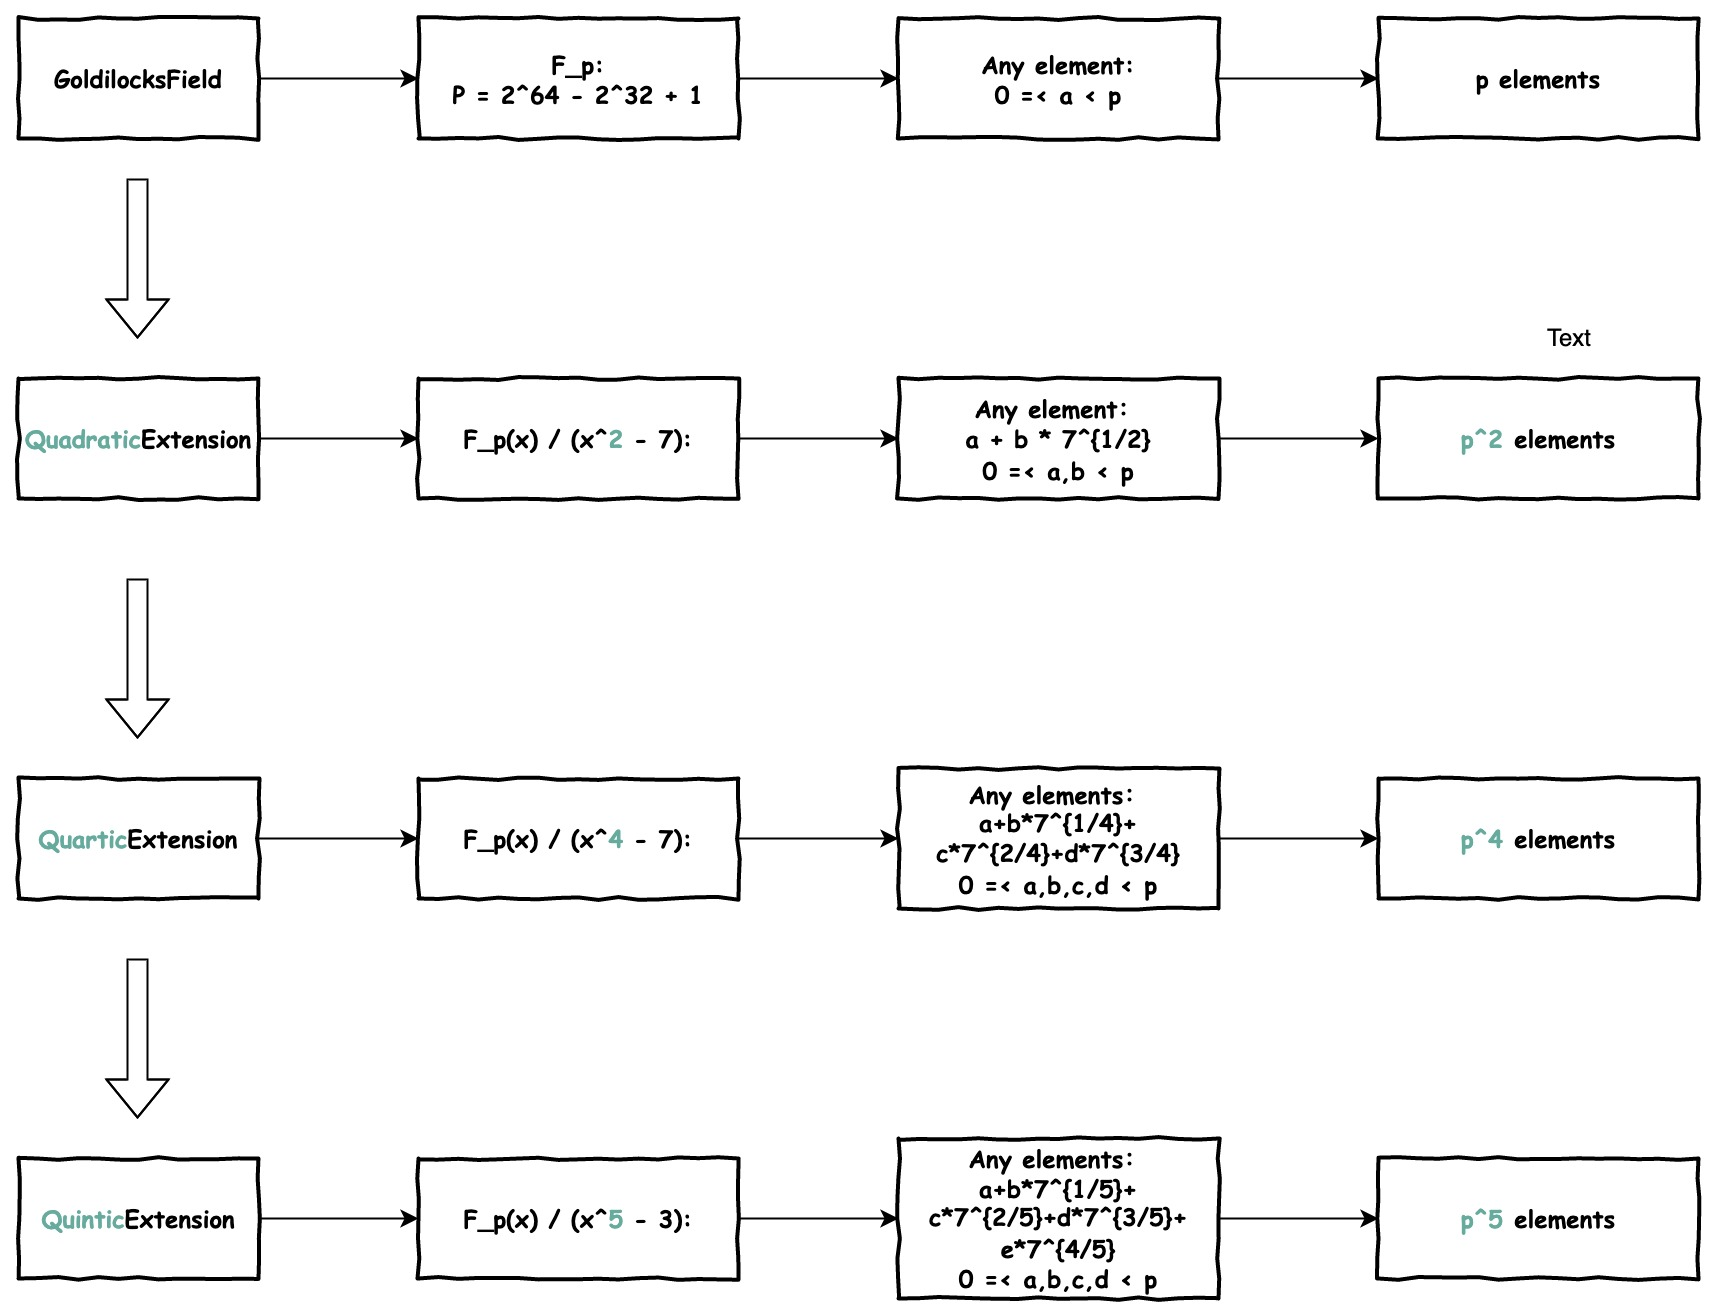
\includegraphics[width=0.8\textwidth]{gates/arthmetic_extension_ext.jpeg}
    \caption{GoldilocksField Extension}
    \label{fig:goldilocksfield-extension}
\end{figure}

It is easy to see that for QuadraticExtension Field, the elements on its domain take the form $a + b \sqrt{7}; a,b \subset F_p$, and a, b cannot both be 0.
It can be seen that on the quadratic extension domain, there are $p^2$ elements and the original domain is a subset of the quadratic extension domain.

ArithmeticExtensionGate is also a gate which can perform a weighted multiply-add, i.e.
\[res = cons\_0 * mul\_0 * mul\_1 + cons\_1 * add\]
The elements of the QuadraticExtension Field are represented in the form $[a, b]$, so the Gate design for arithmetic\_extension has the following form:

\begin{figure}[!ht]
    \centering
    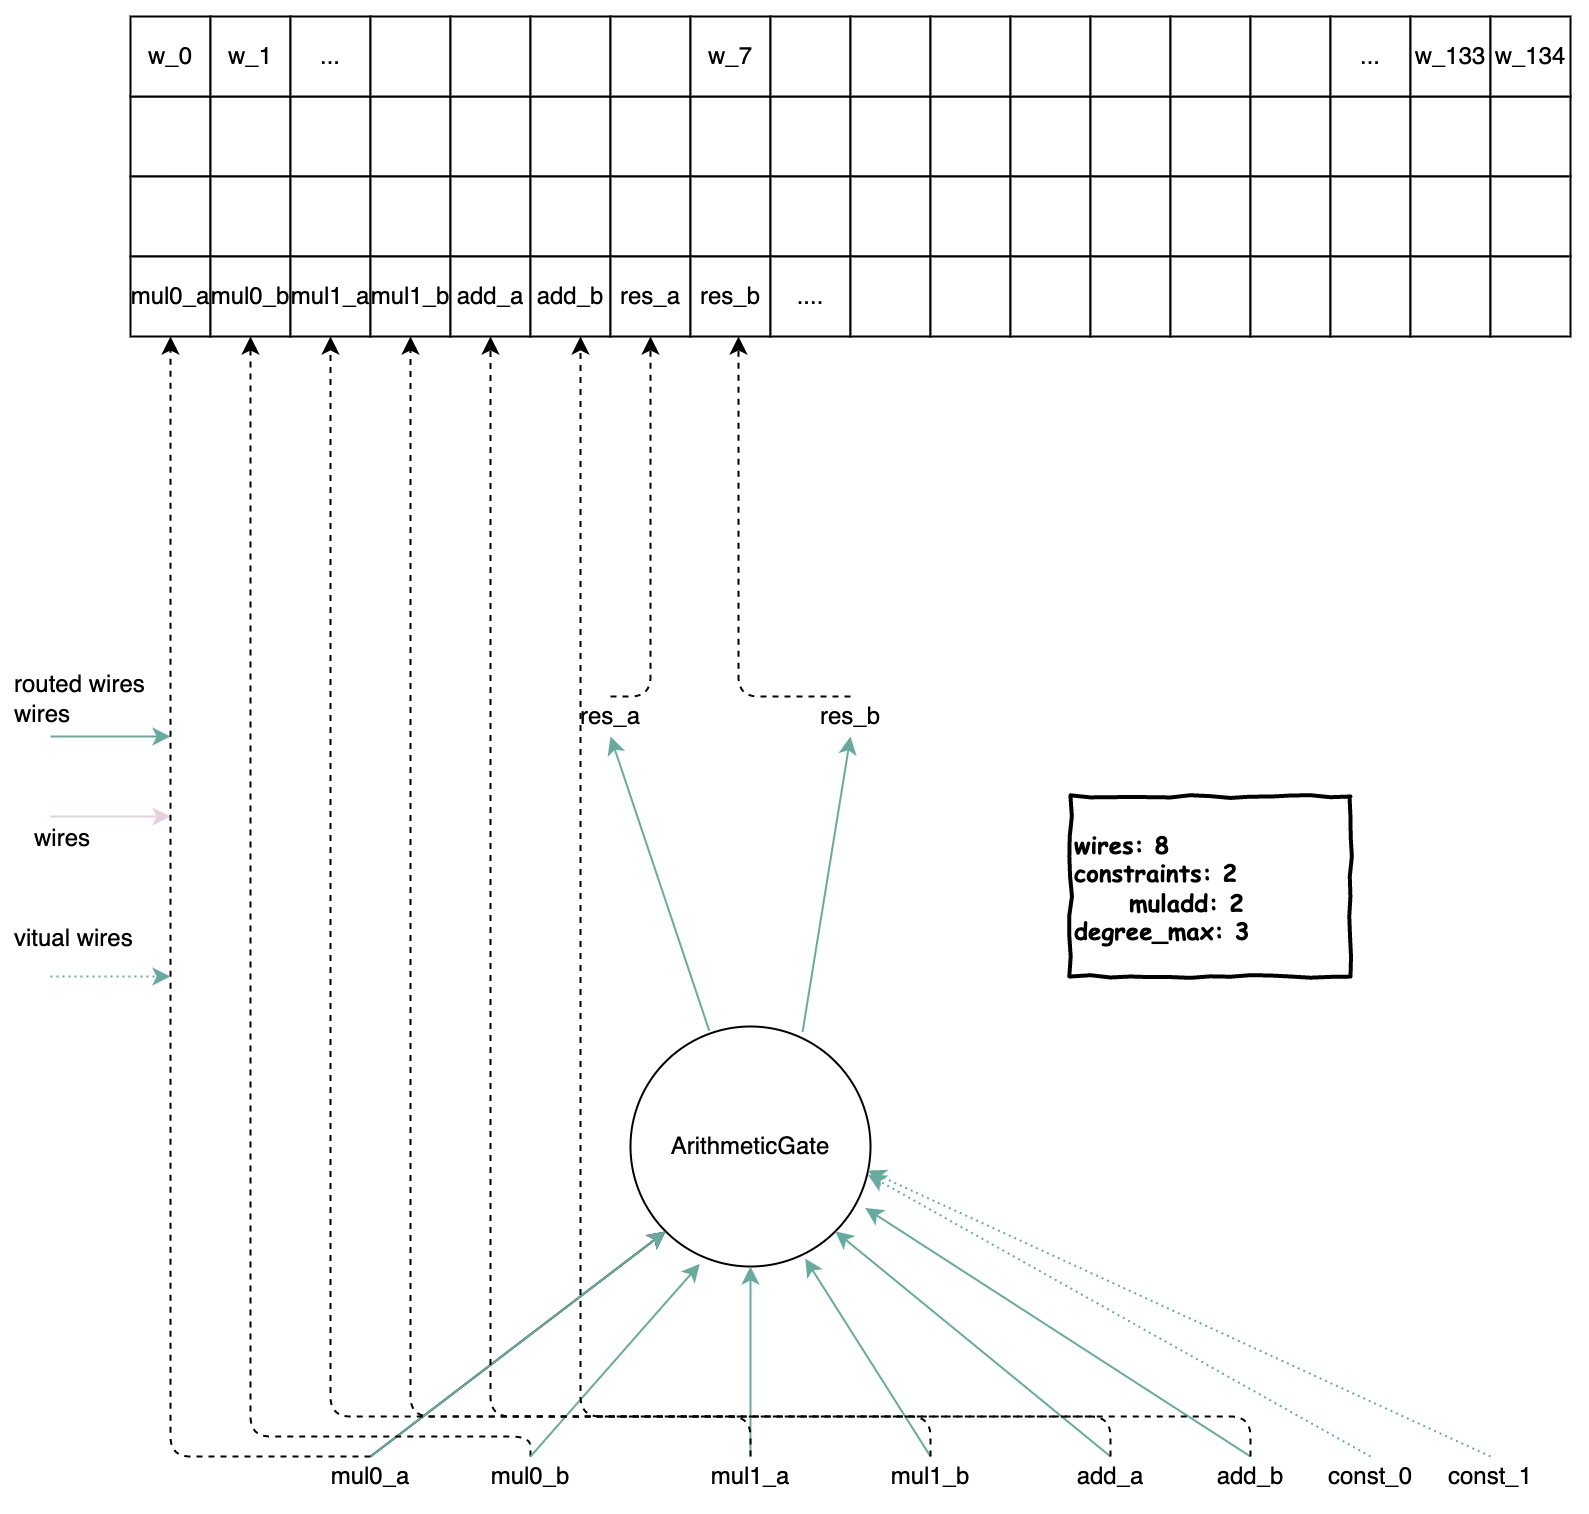
\includegraphics[width=0.8\textwidth]{gates/arthmetic_extension.jpeg}
    \caption{ArithmeticExtensionGate}
    \label{fig:arthmetic-extension}
\end{figure}